\chapter{Model Skalar Cahaya}\label{ch:b2:scalar-light-model}

Sorotkanlah dua senter ke dinding yang sama dan bercaknya sekadar dua kali
lebih terang; sorotkanlah dua berkas dari satu laser ke sana dan bercaknya pecah menjadi
rumbai terang dan gelap. Senternya menjumlahkan intensitasnya, berkas lasernya
menjumlahkan amplitudonya --- dan setiap interferometer, hologram dan
kisi difraksi bab yang akan datang bersandar pada pengetahuan kapan cahaya
melakukan yang mana. Bab ini menyiapkan perkakasnya: cahaya sebagai gelombang
\emph{skalar} berfase, \emph{\omterm{def:b2:scalar-light-model:path}{lintasan optik}} yang mengukur fase itu
sepanjang sebuah sinar, cara sebuah sumber memancar --- ringkasnya \omterm{prop:b2:scalar-light-model:coherence}{deret gelombang} yang
\emph{\omterm{prop:b2:scalar-light-model:coherence}{panjang koherensi}}-nya memutuskan dapat tidaknya dua gelombang berinterferensi --- dan
cara sebuah detektor merekamnya: sebuah rerata sepanjang bermiliar periode
yang hanya menyimpan intensitasnya.

\section{Cahaya sebagai gelombang skalar}

\begin{definition}[Model skalar; gelombang monokromatik]\label{def:b2:scalar-light-model:scalar}
\index{model skalar cahaya}\index{getaran (optik)}\index{gelombang monokromatik}
Dalam sebagian besar optika gelombang sifat vektor cahaya tak berperan (gelombang
yang ditumpangkan berbagi satu polarisasi, atau cahayanya tak terpolarisasi
sehingga polarisasinya saling merata): medannya diganti sebuah
\emph{getaran skalar} nyata
\[
s(M, t) = a(M)\cos\bigl(\omega t - \varphi(M)\bigr) ,
\]
dengan amplitudo $a(M)$ dan fase $\varphi(M)$ di tiap titiknya, keduanya
berubah lambat pada skala satu panjang gelombang. Gelombang \emph{monokromatik}
mempunyai satu $\omega$ saja: sebuah pengidealan, sebab sumber yang sungguhan memancar
pada sebuah pita frekuensi. Cahaya tampak: $\lambda_0$ dari $400$ sampai
\qty{750}{nm} dalam hampa, $\nu = c/\lambda_0$ dari $7.5 \times 10^{14}$ sampai $4 \times 10^{14}$ Hz,
periodenya sekitar \qty{2}{fs}.
\end{definition}

\begin{definition}[Lintasan optik dan fase]\label{def:b2:scalar-light-model:path}
\index{lintasan optik}\index{fase (optik)}\index{muka gelombang}\index{teorema Malus--Dupin}
Dalam medium berindeks $n$ gelombangnya berjalan dengan $c/n$ dan panjang gelombangnya
adalah $\lambda_0/n$. \emph{Lintasan optik} sepanjang sebuah kurva dari $A$ ke $B$ adalah
\[
(AB) = \int_A^Bn\,\dd s ,
\]
dan fase yang dihimpun sebuah \omterm{def:b2:scalar-light-model:scalar}{gelombang monokromatik} yang berjalan sepanjang
sebuah sinar dari $A$ ke $B$ adalah
\[
\varphi(B) - \varphi(A) = \frac{2\pi}{\lambda_0}\,(AB) = \omega\,\tau_{AB} ,
\]
dengan $\tau_{AB}$ yaitu waktu tempuhnya. \emph{Muka gelombang} adalah permukaan
berfase sama; dalam medium isotropik sinar optika geometri
tegak lurus muka gelombangnya (teorema Malus--Dupin), dan lintasan
optik antara dua muka gelombang sama sepanjang setiap sinarnya.
\end{definition}

\begin{proof}[Pembenaran]
Fasenya maju sebesar $2\pi$ tiap panjang gelombang setempat $\lambda_0/n$, yakni sebesar
$2\pi n\,\dd s/\lambda_0$ tiap elemen $\dd s$; dijumlahkan sepanjang sinarnya. Gelombang
$a\cos(\omega t - \varphi)$ adalah penyelesaian \omterm{thm:b2:waves-on-strings:equation}{persamaan gelombang} yang di dalamnya
energinya berjalan sepanjang $\operatorname{\vect{grad}}\varphi$, tegak lurus
permukaan $\varphi =$ tetap: itulah sinarnya, dan pernyataan ``\omterm{def:b2:scalar-light-model:path}{lintasan optik} = sama
antara dua \omterm{def:b2:scalar-light-model:path}{muka gelombang}'' adalah definisi \omterm{def:b2:scalar-light-model:path}{muka gelombang}
yang dibaca terbalik. Teorema penuhnya (ia bertahan menembus pemantulan dan
pembiasan) diterima tanpa bukti.
\end{proof}

\begin{example}[Stigmatisme; lensa sebagai keping fase]\label{ex:b2:scalar-light-model:lens}
\index{stigmatisme}\index{lensa tipis (fase)}
Sebuah sumber titik $A$ yang dicitrakan sebuah instrumen sempurna (stigmatik) di $A'$:
semua sinar dari $A$ ke $A'$ mempunyai \emph{\omterm{def:b2:scalar-light-model:path}{lintasan optik} yang sama} ---
gelombang yang tiba sepanjang setiap sinarnya sefase di $A'$, itulah sebabnya mereka
menumpuk menjadi sebuah titik terang di sana. Bagi lensa tipis berjarak fokus $f$
ini merupakan pernyataan tentang fase: sebuah gelombang bidang yang tiba sepanjang sumbunya
harus pergi sebagai \omterm{prop:b2:sound-waves:spherical}{gelombang bola} yang memusat ke fokusnya $F'$; karena sebuah
\omterm{prop:b2:sound-waves:spherical}{gelombang bola} yang berpusat pada jarak $f$ mempunyai, pada jarak $r$ dari sumbunya,
fase $2\pi r^2/2\lambda f$ mendahului nilai sesumbunya (hampiran
paraksial, $\sqrt{f^2 + r^2} \approx f + r^2/2f$), lensanya harus
\emph{menunda} gelombangnya sebesar $\varphi_L(r) = -\pi r^2/\lambda f$: ia lebih tebal di
tengahnya tepat sebesar yang membuat semua \omterm{def:b2:scalar-light-model:path}{lintasan optik} ke $F'$
sama. Sebuah lensa adalah keping fase; sebuah hologram atau paparan kristal cair
yang memaksakan peta fase yang sama adalah sebuah lensa.
\end{example}

\begin{omfigure}
\begin{tikzpicture}[font=\small, x=1cm, y=1cm, >=Stealth]
  \begin{scope}
    \foreach \x in {-3.0,-2.4,-1.8} \draw[omDef, thick] (\x,-1.5) -- (\x,1.5);
    \draw[thick, fill=omExo!20] (0,0) ellipse (0.25 and 1.6);
    \draw[omDef, thick] (1.0,1.25) arc[start angle=125, end angle=235, x radius=1.9, y radius=1.5];
    \draw[omDef, thick] (1.7,1.0) arc[start angle=130, end angle=230, x radius=1.4, y radius=1.3];
    \draw[omDef, thick] (2.35,0.7) arc[start angle=135, end angle=225, x radius=1.0, y radius=1.0];
    \fill (3.2,0) circle (1.6pt); \node[font=\footnotesize] at (3.4,-0.3) {$F'$};
    \draw[omThm, ->] (-3.2,0.9) -- (-0.4,0.9); \draw[omThm, ->] (0.3,0.9) -- (3.1,0.05);
    \draw[omThm, ->] (-3.2,-0.9) -- (-0.4,-0.9); \draw[omThm, ->] (0.3,-0.9) -- (3.1,-0.05);
    \draw[omThm, ->] (-3.2,0) -- (3.1,0);
    \node[font=\footnotesize] at (0,-2.1) {muka gelombang bidang $\to$ bola: lensanya menunda tengahnya};
  \end{scope}
  \begin{scope}[xshift=9.0cm]
    \fill[omExo!20] (-1.0,-1.4) rectangle (1.0,1.4); \draw[thick] (-1.0,-1.4) -- (-1.0,1.4) (1.0,-1.4) -- (1.0,1.4);
    \foreach \x in {-2.8,-2.2,-1.6} \draw[omDef, thick] (\x,-1.2) -- (\x,1.2);
    \foreach \x in {-0.7,-0.3,0.1,0.5,0.9} \draw[omDef, thick] (\x,-1.2) -- (\x,1.2);
    \foreach \x in {1.6,2.2,2.8} \draw[omDef, thick] (\x,-1.2) -- (\x,1.2);
    \node[font=\footnotesize] at (0,1.7) {$n$: $\lambda_0/n$}; \node[font=\footnotesize] at (-2.2,1.7) {$\lambda_0$};
    \node[font=\footnotesize] at (0,-2.1) {lintasan optik $(AB) = \int n\,\dd s$};
  \end{scope}
\end{tikzpicture}

{\small Kiri: sebuah lensa tipis mengubah \omterm{def:b2:scalar-light-model:path}{muka gelombang} bidang menjadi bola
yang memusat pada fokusnya --- semua \omterm{def:b2:scalar-light-model:path}{lintasan optik} ke $F'$ sama. Kanan:
di dalam kaca panjang gelombangnya menyusut menjadi $\lambda_0/n$ dan fasenya maju
lebih cepat: \omterm{def:b2:scalar-light-model:path}{lintasan optiknya} mencacah panjang geometrinya $n$ kali.}
\end{omfigure}

\section{Bagaimana cahaya dipancarkan: koherensi}

\begin{proposition}[Deret gelombang; waktu dan panjang koherensi]\label{prop:b2:scalar-light-model:coherence}
\index{deret gelombang}\index{waktu koherensi}\index{panjang koherensi}\index{lebar spektrum}
Sebuah sumber klasik (nyala api, lampu, bintang) adalah kumpulan atom
yang masing-masingnya memancarkan, pada saat acak dan dengan fase acak,
\emph{\omterm{prop:b2:scalar-light-model:coherence}{deret gelombang}} pendek berdurasi $\tau_c$: getaran yang dihasilkannya di sebuah
titik menjaga fase yang mantap hanya sepanjang $\tau_c$ lalu melompat. Sebuah deret
berdurasi $\tau_c$ tidak monokromatik: spektrumnya merentangi pita
frekuensi $\Delta\nu \approx 1/\tau_c$ (sebuah kebalikan Fourier, diterima tanpa bukti: sinusoid
yang berhingga tak dapat berfrekuensi tunggal). \emph{\omterm{prop:b2:scalar-light-model:coherence}{Waktu koherensi}}
$\tau_c$ dan \emph{\omterm{prop:b2:scalar-light-model:coherence}{panjang koherensi}}
\[
\ell_c = c\,\tau_c \approx \frac c{\Delta\nu} = \frac{\lambda^2}{\Delta\lambda}
\]
mencirikan sumbernya: cahaya putih $\Delta\lambda \approx \qty{300}{nm}$, $\ell_c
\approx \qty{1}{\micro m}$; sebuah lampu spektrum ($\Delta\lambda \sim \qty{0.01}{nm}$), $\ell_c \sim
\qty{3}{cm}$; sebuah laser, bermeter sampai berkilometer. Dua gelombang yang diturunkan dari
sumber yang sama hanya dapat berinterferensi jika beda lintasannya lebih kecil
daripada $\ell_c$ --- di luarnya keduanya milik deret yang berbeda, dengan
fase yang tak berhubungan.
\end{proposition}

\begin{proof}
$\ell_c = c/\Delta\nu$ dan $|\Delta\nu/\nu| = |\Delta\lambda/\lambda|$ dengan $\nu = c/\lambda$ memberi $\ell_c =
\lambda^2/\Delta\lambda$. \omterm{prop:b2:scalar-light-model:coherence}{Lebar spektrumnya} sendiri mempunyai sebab fisis: lebar
alaminya (peredaman radiasi, \cref{ch:b2:dipole-radiation}),
pelebaran Doppler oleh gerak termal atomnya, tumbukan --- masing-masingnya
memendekkan deretnya.
\end{proof}

\begin{omfigure}
\begin{tikzpicture}
\begin{axis}[omaxis, axis x line=middle, axis y line=none, width=13.6cm, height=3.6cm,
    xmin=0, xmax=60, ymin=-1.4, ymax=1.6, xtick=\empty, samples=800, xlabel={$t$},
    xlabel style={at={(axis description cs:1.0,0.5)}, anchor=west}]
  \addplot[omDef, thick, domain=0:14] {cos(deg(2.2*x))};
  \addplot[omDef, thick, domain=14:31] {cos(deg(2.2*x)+110)};
  \addplot[omDef, thick, domain=31:42] {cos(deg(2.2*x)+240)};
  \addplot[omDef, thick, domain=42:60] {cos(deg(2.2*x)+40)};
  \draw[omThm, <->] (axis cs:14,1.35) -- (axis cs:31,1.35) node[midway, above, font=\scriptsize] {$\tau_c$};
  \draw[omThm, dashed] (axis cs:14,-1.2) -- (axis cs:14,1.2);
  \draw[omThm, dashed] (axis cs:31,-1.2) -- (axis cs:31,1.2);
  \draw[omThm, dashed] (axis cs:42,-1.2) -- (axis cs:42,1.2);
\end{axis}
\end{tikzpicture}

{\small Getaran dari sebuah sumber klasik: sebuah rentetan \omterm{prop:b2:scalar-light-model:coherence}{deret
gelombang} berdurasi $\tau_c$ dengan lompatan fase acak di antaranya; dua
salinannya hanya dapat berinterferensi jika tundanya lebih pendek daripada $\tau_c$.}
\end{omfigure}

\begin{remark}[Dua sumber, satu sumber]\label{rem:b2:scalar-light-model:twosources}
\index{sumber takkoheren}
Dua lampu yang berbeda (atau dua atom yang berbeda) memancarkan deret dengan
fase acak yang saling bebas: fase nisbinya berubah tiap $\tau_c
\sim \qty{1e-9}{s}$, sejuta kali lebih cepat daripada tanggapan mata atau kamera
mana pun --- suku interferensinya rata-ratanya nol dan
intensitasnya bertambah. Interferensi menuntut dua gelombang yang \emph{mengingat
lompatan fase yang sama}: dua salinan satu gelombang, yang diperoleh dengan membelahnya
(dua celah, dua cermin, kedua muka sebuah selaput) lalu digabungkan kembali dengan
tunda yang lebih pendek daripada $\tau_c$. Sebuah laser, yang deretnya berlangsung bermikrosekon atau
lebih, mengendurkan kendala ini secara luar biasa; ia tak pernah menyingkirkannya.
\end{remark}

\section{Detektor dan intensitas}

\begin{proposition}[Apa yang diukur sebuah detektor]\label{prop:b2:scalar-light-model:intensity}
\index{intensitas (optika)}\index{detektor (optika)}\index{fluks foton}
Setiap detektor cahaya --- mata (waktu tanggapnya $\sim\qty{0.1}{s}$), sebuah
selaput foto, sebuah piksel CCD (\qty{1}{ms}), sebuah fotodioda (\qty{1}{ns}) ---
menanggapi pada waktu yang panjang dibandingkan periodenya ($10^{-15}$ s) lalu
menyerahkan \emph{intensitas}-nya, yaitu rerata waktu kuadrat
getarannya,
\[
I = K\,\langle s^2\rangle = \tfrac12K\,a^2 ,
\]
($K$ sebuah tetapan, sering dibuang; $I$ sebanding dengan iradiansinya
dalam \unit{W/m^2}). Aras mutlaknya berarti hanya dalam satu hal: cahaya
tiba dalam foton berenergi $h\nu$, dan sebuah detektor mencacah rata-rata
$I/h\nu$ foton tiap satuan luas dan waktu.
\end{proposition}

\begin{proof}
$\langle\cos^2(\omega t - \varphi)\rangle = \tfrac12$ sepanjang selang mana pun yang jauh lebih panjang
daripada $2\pi/\omega$. Fotonnya: bab terakhir jilid Tahun 1; di sinilah
gelombang skalarnya berjumpa dengan kuantum.
\end{proof}

\begin{example}[Orde besaran]\label{ex:b2:scalar-light-model:orders}
Sebuah bola lampu \qty{60}{W} yang memancarkan \qty{3}{W} cahaya tampak pada \qty{2}{m}:
$I = 3/4\pi\cdot4 = \qty{60}{mW/m^2}$, $I/h\nu = 1.6 \times 10^{17}$ foton tiap meter
persegi tiap sekon, $3 \times 10^{12}$ tiap sekon menembus pupil \qty{5}{mm} ---
dalam \qty{0.1}{s} milik matanya tak ada jejak kekasarannya. Bintang
paling redup yang dilihat mata mengirimkan $\sim 10^3$ foton tiap sekon ke dalam
pupilnya; sebuah sel batang menyala pada segenggam foton. Cahaya matahari: \qty{1}{kW/m^2}, $3 \times 10^{21}$
foton tiap meter persegi tiap sekon.
\end{example}

\begin{omfigure}
\begin{tikzpicture}[font=\small, x=1cm, y=1cm, >=Stealth]
  \draw[->, thick] (0,0) -- (12.6,0) node[right, font=\footnotesize] {waktu (s)};
  \foreach \x/\l in {0/$10^{-15}$, 2/$10^{-13}$, 4/$10^{-11}$, 6/$10^{-9}$, 8/$10^{-7}$, 10/$10^{-5}$, 12/$10^{-3}$} {
    \draw (\x,-0.1) -- (\x,0.1); \node[font=\scriptsize, below] at (\x,-0.12) {\l};
  }
  \draw[omDef, very thick] (0,0.45) -- (0.4,0.45); \node[omDef, font=\footnotesize, anchor=west] at (0.5,0.45) {periode optik};
  \draw[omThm, very thick] (2.0,0.95) -- (6.0,0.95); \node[omThm, font=\footnotesize, anchor=west] at (6.1,0.95) {deret gelombang (lampu)};
  \draw[omThm, very thick] (6.0,1.45) -- (10.0,1.45); \node[omThm, font=\footnotesize, anchor=west] at (10.1,1.45) {laser};
  \draw[omProp, very thick] (6.0,1.95) -- (12.4,1.95); \node[omProp, font=\footnotesize, anchor=west] at (6.1,2.2) {detektor: fotodioda $\to$ CCD $\to$ mata ($10^{-1}$)};
\end{tikzpicture}

{\small Skala waktu optika: periode getarannya, durasi
\omterm{prop:b2:scalar-light-model:coherence}{deret gelombang} sumber klasik dan laser, dan
waktu tanggap detektornya --- semua detektor merata-ratakan banyak
periode, dan banyak deret sebuah lampu.}
\end{omfigure}

\begin{remark}[Tumpang tindih koheren dan takkoheren]\label{rem:b2:scalar-light-model:superposition}
\index{tumpang tindih koheren}\index{tumpang tindih takkoheren}
Dua getaran $a_1\cos(\omega t - \varphi_1)$ dan $a_2\cos(\omega t - \varphi_2)$ di sebuah
titik memberi $s = s_1 + s_2$ dan
\[
I = \tfrac12K\bigl[a_1^2 + a_2^2 + 2a_1a_2\langle\cos(\varphi_1 - \varphi_2)\rangle\bigr] .
\]
Jika beda fasenya mantap selama pendeteksiannya
(gelombang yang \emph{koheren}): $I = I_1 + I_2 + 2\sqrt{I_1I_2}\cos(\varphi_1 - \varphi_2)$,
yaitu suku interferensinya, yang dipelajari bab berikutnya. Jika ia mengembara
acak (gelombang yang \emph{takkoheren}): $\langle\cos\rangle = 0$ dan $I = I_1 +
I_2$ --- yaitu senternya.
\end{remark}

\begin{method}[Menyiapkan sebuah soal optika]\label{met:b2:scalar-light-model:method}
(1) Tuliskanlah tiap gelombangnya sebagai $a\cos(\omega t - \varphi)$ dengan $\varphi = 2\pi(\text{lintasan optik})/\lambda_0$ dari sumbernya (atau dari sebuah \omterm{def:b2:scalar-light-model:path}{muka gelombang} bersama). (2) Putuskanlah
koherensinya: sumber yang sama, beda lintasan $< \ell_c$? Kalau begitu jumlahkanlah amplitudonya
(notasi kompleks itu nyaman: $\underline s = a\eu^{\iu(\omega t - \varphi)}$, $I =
\tfrac12K|\underline s|^2$); jika tidak jumlahkanlah intensitasnya. (3) Bagi lensa dan
cermin, pakailah \omterm{def:b2:scalar-light-model:path}{lintasan optik} yang sama antara titik sekawannya, atau
gambaran keping fasenya. (4) Ubahlah menjadi apa yang diukur: intensitas,
kontras, cacah foton, lalu periksalah resolusi detektornya dalam waktu
dan ruang.
\end{method}

\section{Latihan}

\begin{exercise}[$\star$]\label{exo:b2:scalar-light-model:1}
Sebuah berkas \qty{600}{nm} menyeberangi \qty{1.0}{cm} kaca ($n = 1.5$). Tentukanlah \omterm{def:b2:scalar-light-model:path}{lintasan
optiknya}; jumlah panjang gelombang di dalamnya; fase tambahan dan tunda tambahannya
dibandingkan dengan \qty{1}{cm} udara; tebal kaca yang menunda
gelombangnya tepat satu panjang gelombang relatif terhadap udara.
\end{exercise}

\begin{exercise}[$\star$]\label{exo:b2:scalar-light-model:2}
Tentukanlah waktu dan \omterm{prop:b2:scalar-light-model:coherence}{panjang koherensi}: cahaya putih ($400$--\qty{750}{nm}); garis lampu
natrium berlebar \qty{0.02}{nm} pada \qty{589}{nm}; sebuah LED merah (\qty{630}{nm},
$\Delta\lambda = \qty{25}{nm}$); sebuah dioda laser beragam banyak ($\Delta\nu = \qty{100}{GHz}$); sebuah
laser terstabilkan ($\Delta\nu = \qty{1}{kHz}$). Mana yang dapat memberi rumbai dengan
beda lintasan \qty{1}{mm}? dengan \qty{10}{m}?
\end{exercise}

\begin{exercise}[$\star$]\label{exo:b2:scalar-light-model:3}
Sebuah penunjuk laser \qty{1}{mW} pada \qty{650}{nm}: tentukanlah foton tiap sekonnya; sebuah
bola lampu \qty{100}{W} (\qty{5}{W} tampak, rerata \qty{550}{nm}) pada \qty{3}{m}: foton tiap
sekon menembus pupil \qty{6}{mm}; jumlahnya selama \qty{0.1}{s} milik matanya;
fluktuasi nisbi $1/\sqrt N$ jumlah itu --- kasarkah cahayanya?
\end{exercise}

\begin{exercise}[$\star$]\label{exo:b2:scalar-light-model:4}
Sebuah sumber titik pada \qty{1.0}{m} dari sebuah layar, $\lambda = \qty{500}{nm}$. Tentukanlah beda
\omterm{def:b2:scalar-light-model:path}{lintasan optik} antara pusat layarnya dan sebuah titik \qty{1}{cm}
dari sumbunya (secara eksak, lalu dengan rumus paraksial $r^2/2d$); jumlah
panjang gelombangnya; jari-jari \omterm{def:b2:scalar-light-model:path}{muka gelombangnya} di layarnya; pada jarak berapa dari sumbunya
rumus paraksialnya salah sebesar satu panjang gelombang?
\end{exercise}

\begin{exercise}[$\star\star$]\label{exo:b2:scalar-light-model:5}
\emph{Lensa sebagai keping fase.} (a) Sebuah gelombang bidang sepanjang sumbunya mempunyai
fase yang seragam pada bidang sebuah lensa tipis; sesudah lensanya fasenya
$\varphi_L(r) = -\pi r^2/\lambda f$ relatif terhadap tengahnya. Tunjukkanlah bahwa \omterm{def:b2:scalar-light-model:path}{muka gelombang}
yang muncul, dalam hampiran paraksial, adalah sebuah bola berjari-jari $f$
berpusat pada $F'$. (b) Sebuah sumber titik pada jarak $d$ di depan lensanya
mengirimkan gelombang yang fasenya pada bidang lensanya adalah $+\pi r^2/\lambda d$ (relatif terhadap
tengahnya): tunjukkanlah bahwa sesudah lensanya gelombangnya memusat di $d'$ dengan
$1/d' = 1/f - 1/d$, yaitu rumus lensanya. (c) Profil tebal sebuah
lensa kaca plano-cembung ($n = 1.5$) berjarak fokus \qty{10}{cm}: $e(r) =
e_0 - r^2/2(n - 1)f$; berapa lendutannya di $r = \qty{1}{cm}$. (d) Sebuah ``lensa Fresnel'' melipat
profilnya kembali tiap kali ia melampaui $\lambda/(n - 1)$: mengapa ia masih
memfokus, dan mengapa hanya satu warna dengan sempurna?
\end{exercise}

\begin{exercise}[$\star\star$]\label{exo:b2:scalar-light-model:6}
\emph{Stigmatisme sebuah cermin.} Sebuah cermin harus mengirimkan gelombang bidang yang tiba
sepanjang sumbunya ke sebuah titik $F$. (a) Tuliskanlah syarat ``\omterm{def:b2:scalar-light-model:path}{lintasan optik}
yang sama dari sebuah \omterm{def:b2:scalar-light-model:path}{muka gelombang} bidang ke $F$ bagi setiap titik cerminnya'' lalu
tunjukkanlah bahwa ia mendefinisikan sebuah parabola $y^2 = 4fx$ dengan $F$ di fokusnya. (b) Mengapa sebuah
cermin bola hanya stigmatik secara hampiran (bandingkanlah $y^2 = 4fx$ dengan
lingkaran berjari-jari $2f$ dekat puncaknya)? (c) Bagi cermin \qty{20}{cm}
ber-$f = \qty{1}{m}$, berapa galat lintasan bolanya di tepinya, dalam
panjang gelombang \qty{500}{nm}. (d) Mengapa teleskop radio memaklumi
kebolaan yang tak dapat dimaklumi teleskop optik?
\end{exercise}

\begin{exercise}[$\star\star$]\label{exo:b2:scalar-light-model:7}
\emph{Fermat.} \omterm{def:b2:scalar-light-model:path}{Lintasan optik} dari $A$ (dalam medium $n_1$) ke $B$ (dalam
$n_2$) menembus sebuah titik $P$ pada antarmuka bidangnya adalah $n_1AP + n_2PB$. (a)
Tunjukkanlah bahwa ia tegar (terkecil) bagi titik $P$ yang memenuhi
$n_1\sin\theta_1 = n_2\sin\theta_2$. (b) Tafsirkanlah: lintasan tetangganya berfase
sama, sehingga gelombang sepanjangnya bertambah --- inilah sebabnya cahaya
``memilih'' sinar Descartesnya. (c) Turunkanlah hukum pemantulannya dengan cara
yang sama. (d) Mengapa lintasan menembus sebuah lensa dari $A$ ke citranya $A'$ sama
sepanjang setiap sinarnya, dan bukan sekadar tegar?
\end{exercise}

\begin{exercise}[$\star\star$]\label{exo:b2:scalar-light-model:8}
\emph{Mengapa dua lampu tidak berinterferensi.} Dua lampu natrium menyinari sebuah
layar; di sebuah titik, gelombangnya beramplitudo $a$ dan berbeda
fase $\Delta\varphi$ yang melompat acak tiap $\tau_c = \qty{1e-10}{s}$. (a)
Tentukanlah intensitas di titik itu sebagai fungsi $\Delta\varphi$; maksimum dan
minimumnya. (b) Detektornya merata-ratakan sepanjang $\tau_d = \qty{1}{ms}$: berapa banyak
nilai $\Delta\varphi$ yang saling bebas? Tentukanlah intensitas reratanya; ukuran nisbi
fluktuasi sisa suku interferensinya ($\sim 1/\sqrt N$). (c) Sebuah
fotodioda ber-$\tau_d = \qty{1e-11}{s}$: apa yang akan dilihatnya? (d) Bagaimana
percobaan pertama yang menunjukkan interferensi antara dua laser yang saling bebas
(1963) menanganinya?
\end{exercise}

\begin{exercise}[$\star\star$]\label{exo:b2:scalar-light-model:9}
\emph{Kedalaman semu.} Sekeping uang logam terletak pada kedalaman $h$ dalam air ($n = 1.33$).
(a) Dengan memakai \omterm{def:b2:scalar-light-model:path}{lintasan optiknya} (atau hukum Descartes pada sudut kecil), tunjukkanlah
bahwa sebuah mata di atasnya melihatnya pada kedalaman $h/n$. (b) $h = \qty{1.2}{m}$: tentukanlah kedalaman
semunya; seberapa besar \omterm{def:b2:scalar-light-model:path}{lintasan optik} dari uang logamnya ke matanya
melampaui panjang geometrinya? (c) Seekor ikan pada kedalaman $h$ melihat seekor lalat \qty{1}{m}
di atas permukaannya pada ketinggian semu berapa? (d) Mengapa sebuah kolam tampak
lebih dangkal lagi ketika dipandang miring?
\end{exercise}

\begin{exercise}[$\star\star\star$]\label{exo:b2:scalar-light-model:10}
\emph{Kontras dan koherensi.} Dua salinan sebuah gelombang berbeda lintasan
$\delta$ ditumpangkan; spektrum sumbernya tersebar
seragam pada $[\nu_0 - \Delta\nu/2, \nu_0 + \Delta\nu/2]$, dan tiap frekuensinya
hanya berinterferensi dengan dirinya sendiri. (a) Intensitas dari satu frekuensi: $2I_0
[1 + \cos(2\pi\nu\delta/c)]$. (b) Integralkanlah pada pitanya lalu tunjukkanlah bahwa
totalnya adalah $2I_0[1 + \operatorname{sinc}(\pi\Delta\nu\,\delta/c)\cos(2\pi\nu_0\delta/c)]$ dengan
$\operatorname{sinc}x = \sin x/x$. (c) Definisikanlah kontras $V = (I_{\max} -
I_{\min})/(I_{\max} + I_{\min})$ rumbainya dekat $\delta$ lalu tunjukkanlah $V =
|\operatorname{sinc}(\pi\Delta\nu\,\delta/c)|$: ia lenyap pada $\delta = c/\Delta\nu = \ell_c$. (d)
Angkanya bagi sebuah LED ($\Delta\lambda = \qty{25}{nm}$ pada \qty{630}{nm}): pada $\delta$ berapa
kontrasnya lenyap pertama kali.
\end{exercise}

\begin{exercise}[$\star\star\star$]\label{exo:b2:scalar-light-model:11}
\emph{Melihat bintang.} Mata mendeteksi sebuah kilatan ketika sekitar $10$ foton
mencapai sebuah sel batang dalam \qty{0.1}{s}; pupil yang teradaptasi gelap adalah \qty{7}{mm}; ambillah
\qty{500}{nm}. (a) Tentukanlah \omterm{prop:b2:scalar-light-model:intensity}{fluks foton} dan iradiansi minimum di matanya. (b)
Matahari memberi \qty{1}{kW/m^2}; sebuah bintang bermagnitudo $m$ memberi $10^{-0.4(m + 26.7)}$
darinya: tentukanlah iradiansi sebuah bintang bermagnitudo 6 (batas mata telanjang) dan
laju fotonnya ke dalam pupilnya; selaraskah dengan (a)? (c) Sebuah teleskop
berapertur \qty{200}{mm}: berapa perolehan fotonnya, dan magnitudo yang dicapainya.
(d) Mengapa ahli astronomi berbicara tentang ``derau foton'' sebuah citra yang redup,
dan bagaimana ia berskala dengan waktu pajanannya?
\end{exercise}

\begin{exercise}[$\star\star\star$]\label{exo:b2:scalar-light-model:12}
\emph{Melampaui paraksial.} Sebuah \omterm{prop:b2:sound-waves:spherical}{gelombang bola} dari sebuah titik pada jarak $d$
mempunyai, pada jarak melintang $r$, lintasan tambahan eksak $\sqrt{d^2 +
r^2} - d$. (a) Uraikanlah sampai orde empat: $r^2/2d - r^4/8d^3$. (b) Suku
kuadratik (paraksial)-nya disimpan dan yang kuartik dibuang ketika
yang terakhir di bawah $\lambda/4$: tunjukkanlah bahwa ini menuntut $r^4 < 2\lambda d^3$. (c) Angkanya:
$d = \qty{1}{m}$, $\lambda = \qty{500}{nm}$: berapa $r$ maksimumnya; $d = \qty{1}{cm}$ (sebuah mikroskop):
berapa $r$ maksimumnya, dan sudut yang bersesuaian. (d) Ulasan: yang disebut
``aberasi'' optika geometri adalah suku yang terabaikan ini.
\end{exercise}

\begin{omfigure}
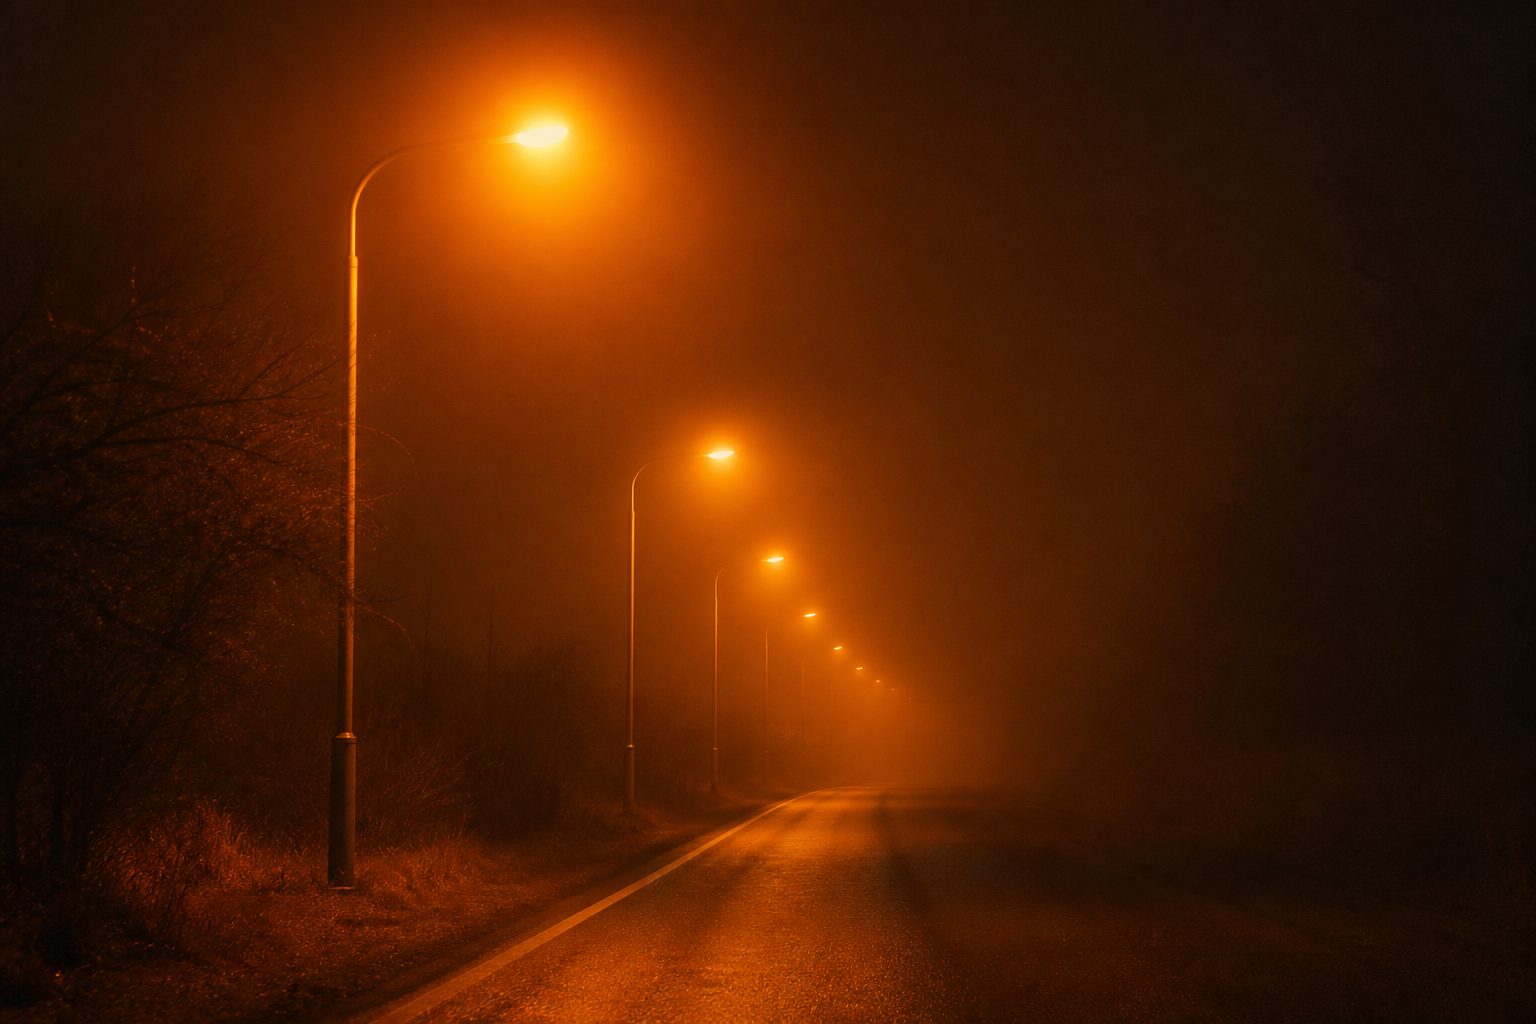
\includegraphics[width=0.58\linewidth]{images/book4/ai/b4-18-sodium-lamps-fog.png}

{\small Lampu natrium bertekanan rendah dalam kabut: satu garis kuning saja, \omterm{prop:b2:scalar-light-model:coherence}{panjang koherensi} bersentimeter --- yaitu sumber klasik laboratorium optika, dan jalanan tua.}
\end{omfigure}

\section{Soal: Sebuah lampu natrium dan sebuah penunjuk laser}

\begin{problem}[{Soal akhir pekan --- dua sumber cahaya yang dibongkar:
lampu kuning jalanan tua, penunjuk merah di ruang kuliah, dan
satu angka yang memutuskan dapat tidaknya masing-masingnya membuat rumbai}]
\label{pb:b2:scalar-light-model:1}

\medskip
\noindent\textbf{Bagian I --- Lampu natriumnya.}
Natrium memancarkan dublet kuningnya pada $\lambda_1 = \qty{589.0}{nm}$ dan $\lambda_2 =
\qty{589.6}{nm}$. Lebar alami tiap garisnya adalah $\Delta\nu_{\text{alami}} =
\qty{10}{MHz}$; dalam lampunya atomnya berada pada \qty{500}{K} (massa natrium
\qty{23}{u}, $k_B = \qty{1.38e-23}{J/K}$, $u = \qty{1.66e-27}{kg}$).
\begin{enumerate}
  \item Frekuensi kedua garisnya dan selisihnya.
  \item \omterm{prop:b2:scalar-light-model:coherence}{Panjang koherensi} satu garisnya seandainya hanya lebar alaminya
        yang berperan.
  \item Pelebaran Doppler: sebuah atom yang bergerak dengan $v$ sepanjang garis
        pandangnya memancar pada $\nu(1 + v/c)$; dengan kelajuan rms termalnya $\sqrt{k_BT
        /m}$ sepanjang satu sumbu, taksirlah $\Delta\nu_D$ lalu bandingkanlah dengan
        lebar alaminya.
  \item \omterm{prop:b2:scalar-light-model:coherence}{Panjang koherensi} satu garis yang melebar Doppler; dalam lampu
        bertekanan tinggi yang sungguhan tumbukan melebarkan garisnya sepuluh kali
        lagi: berapa \omterm{prop:b2:scalar-light-model:coherence}{panjang koherensinya} kemudian.
  \item Kedua garisnya bersama-sama: pada beda lintasan berapa sistem
        rumbainya beranjak dari berimpit ke berlawanan lalu kembali
        (``panjang layangan'' $\lambda^2/\Delta\lambda$)? Itu berapa rumbai?
  \item Seorang mahasiswa membuat interferometer dua berkas dengan lampunya lalu
        menaikkan beda lintasannya dari nol: lukiskanlah
        kontras yang terlihat --- layangannya dan pemadaman akhirnya --- dengan
        angka yang telah ditemukan.
  \item Lampunya memancarkan \qty{1}{W} cahaya kuning: tentukanlah foton tiap sekonnya;
        energi satu fotonnya dalam eV, dan mengapa cahayanya kuning.
  \item Dua lampu natrium berdampingan: dapatkah cahayanya berinterferensi?
        Mengapa pertanyaannya berbeda bagi kedua garis satu lampu?
\end{enumerate}

\medskip
\noindent\textbf{Bagian II --- Penunjuk lasernya.}
Sebuah dioda laser merah \qty{1}{mW} pada \qty{650}{nm} memancarkan, ketika murah, beberapa
ragam membujur yang tersebar pada $\Delta\lambda = \qty{0.5}{nm}$; yang beragam tunggal dan
terstabilkan mempunyai $\Delta\nu = \qty{1}{MHz}$.
\begin{enumerate}[resume]
  \item \omterm{prop:b2:scalar-light-model:coherence}{Panjang koherensi} kedua penunjuknya.
  \item Foton yang dipancarkan tiap sekon; jarak rerata antara foton sepanjang
        berkasnya (dalam meter); bandingkanlah dengan \omterm{prop:b2:scalar-light-model:coherence}{panjang koherensinya} ---
        apa yang dikatakannya tentang ``foton yang berinterferensi''?
  \item Ubahlah sebaran \qty{0.5}{nm} itu menjadi lebar frekuensi; rongga
        diodanya panjangnya \qty{1}{mm} dengan $n = 3.5$: tentukanlah jarak antara ragam
        membujurnya ($c/2nL$) dan jumlah ragam dalam sebarannya.
  \item Berkasnya (berdiameter \qty{1}{mm}) jatuh pada sebuah fotodioda yang
        tiap fotonnya menghasilkan sebuah elektron: berapa arusnya.
  \item Penunjuk murahnya dipakai dalam interferometer dua berkas dengan
        beda lintasan \qty{2}{mm}: ada rumbai atau tidak? Dan yang terstabilkan
        dengan \qty{10}{m}?
  \item Keluaran diodanya sebenarnya dihidupkan dan dimatikan dalam
        pulsa \qty{1}{ns}: dapatkah pulsa dari dua periode berturut-turut
        saling berinterferensi? Apa yang menetapkan koherensinya di sini,
        panjang pulsanya atau lebar garisnya?
  \item Mengapa cahaya sebuah laser tampak ``berbercak'' pada dinding, dan mengapa
        cahaya lampunya tidak?
  \item Sebuah LED merah pada \qty{650}{nm} mempunyai $\Delta\lambda = \qty{25}{nm}$: berapa \omterm{prop:b2:scalar-light-model:coherence}{panjang
        koherensinya}; mengapa sebagian proyektor lebih menyukai LED daripada laser?
\end{enumerate}

\medskip
\noindent\textbf{Bagian III --- \omterm{def:b2:scalar-light-model:path}{Lintasan optik} dan detektor.}
\begin{enumerate}[resume]
  \item Sebuah kaca objek \qty{2}{mm} ($n = 1.5$) disisipkan pada salah satu lengan
        interferometernya: tentukanlah \omterm{def:b2:scalar-light-model:path}{lintasan optik} tambahannya, dan jumlah
        rumbai yang bergeser melewati sebuah tanda.
  \item Kaca objeknya dimiringkan \qty{10}{\degree}: tentukanlah lintasan tambahannya (pakailah $e/\cos r$
        bagi panjangnya dalam kacanya, dikurangi udara yang digantikannya, sampai
        hampiran orde pertama $e(n/\cos r - \cos(i - r)/\cos r)$ --- atau sekadar
        taksirlah dengan lintasan geometri yang lebih panjang); orde besaran
        geseran rumbainya.
  \item Detektornya adalah sebuah kamera berpiksel \qty{10}{\micro m}; rumbainya
        terpisah \qty{50}{\micro m}: berapa piksel tiap rumbainya, dan apa yang
        terjadi pada kontras terukurnya jika jaraknya turun menjadi
        \qty{10}{\micro m}?
  \item Pajanan \qty{10}{ms} pada \qty{1}{\micro W/cm^2} di sebuah piksel: tentukanlah foton tiap
        pikselnya; derau foton nisbinya.
  \item Dua gelombang koheren yang sama berintensitas $I_0$ berjumpa dengan beda
        lintasan $\delta$: tuliskanlah intensitasnya $I(\delta)$ dan periode
        rumbainya dalam $\delta$.
  \item Rumbainya melintas sebuah titik pada \qty{1}{kHz} (sebuah cermin yang
        bergetar): apa yang dilihat mata, apa yang dilihat fotodiodanya?
  \item Lengan interferometernya menembus \qty{10}{m} udara ($n - 1 =
        \qty{2.9e-4}{}$): tentukanlah \omterm{def:b2:scalar-light-model:path}{lintasan optiknya} yang melebihi hampa, dalam rumbai;
        apa yang dilakukan perubahan \qty{1}{\%} tekanan udaranya terhadap polanya.
  \item Lampunya dan penunjuknya memberi \qty{1}{\micro W/cm^2} yang sama: mana
        yang memberi lebih banyak foton tiap sekon, dan mengapa itu tak berarti bagi
        rumbainya?
  \item Ringkaslah: bagi tiap sumbernya, \omterm{prop:b2:scalar-light-model:coherence}{panjang koherensinya}, apa yang membatasinya,
        dan beda lintasan interferometer yang dibolehkannya.
\end{enumerate}
\end{problem}
